% Created by tikzDevice version 0.12.6 on 2026-08-08 02:44:45
% !TEX encoding = UTF-8 Unicode
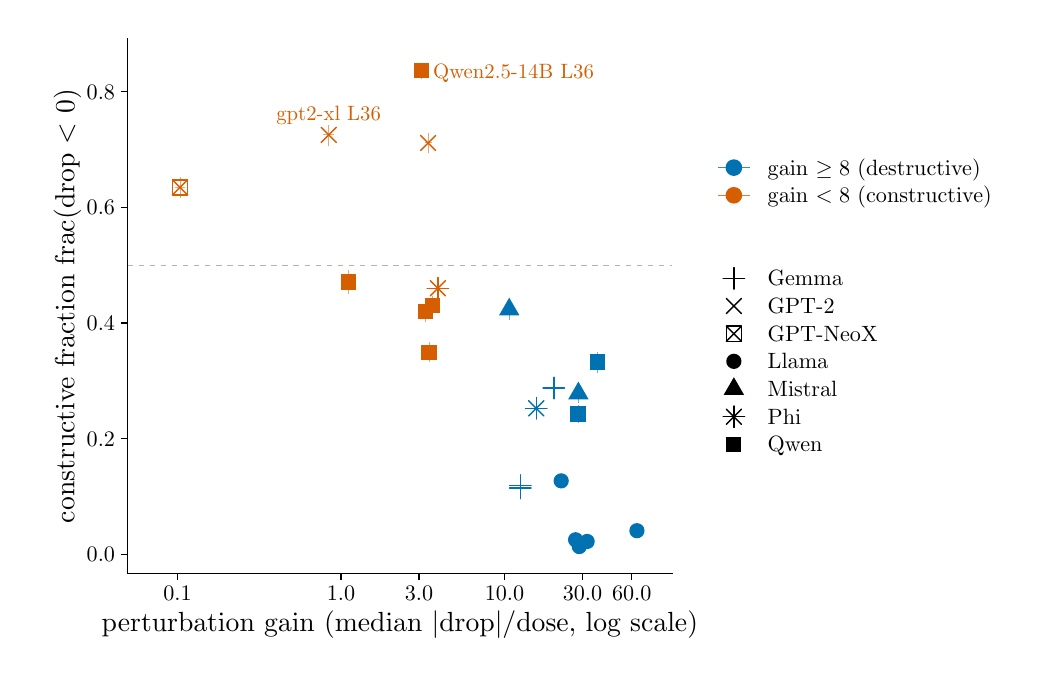
\begin{tikzpicture}[x=1pt,y=1pt]
\definecolor{fillColor}{RGB}{255,255,255}
\path[use as bounding box,fill=fillColor,fill opacity=0.00] (0,0) rectangle (361.35,224.04);
\begin{scope}
\path[clip] (  0.00,  0.00) rectangle (361.35,224.04);
\definecolor{drawColor}{RGB}{255,255,255}
\definecolor{fillColor}{RGB}{255,255,255}

\path[draw=drawColor,line width= 0.5pt,line join=round,line cap=round,fill=fillColor] (  0.00,  0.00) rectangle (361.35,224.04);
\end{scope}
\begin{scope}
\path[clip] ( 36.05, 26.90) rectangle (232.96,220.04);
\definecolor{fillColor}{RGB}{255,255,255}

\path[fill=fillColor] ( 36.05, 26.90) rectangle (232.96,220.04);
\definecolor{drawColor}{gray}{0.70}

\path[draw=drawColor,line width= 0.3pt,dash pattern=on 2pt off 2pt ,line join=round] ( 36.05,138.23) -- (232.96,138.23);
\definecolor{drawColor}{RGB}{0,114,178}

\path[draw=drawColor,draw opacity=0.55,line width= 0.3pt,line join=round] (192.78, 62.72) --
	(192.78, 62.72);

\path[draw=drawColor,draw opacity=0.55,line width= 0.3pt,line join=round] (192.78, 62.72) --
	(192.78, 57.77);

\path[draw=drawColor,draw opacity=0.55,line width= 0.3pt,line join=round] (192.78, 57.77) --
	(192.78, 57.77);

\path[draw=drawColor,draw opacity=0.55,line width= 0.3pt,line join=round] (197.99, 40.25) --
	(197.99, 40.25);

\path[draw=drawColor,draw opacity=0.55,line width= 0.3pt,line join=round] (197.99, 40.25) --
	(197.99, 37.82);

\path[draw=drawColor,draw opacity=0.55,line width= 0.3pt,line join=round] (197.99, 37.82) --
	(197.99, 37.82);

\path[draw=drawColor,draw opacity=0.55,line width= 0.3pt,line join=round] (199.33, 37.43) --
	(199.33, 37.43);

\path[draw=drawColor,draw opacity=0.55,line width= 0.3pt,line join=round] (199.33, 37.43) --
	(199.33, 35.68);

\path[draw=drawColor,draw opacity=0.55,line width= 0.3pt,line join=round] (199.33, 35.68) --
	(199.33, 35.68);

\path[draw=drawColor,draw opacity=0.55,line width= 0.3pt,line join=round] (220.15, 43.82) --
	(220.15, 43.82);

\path[draw=drawColor,draw opacity=0.55,line width= 0.3pt,line join=round] (220.15, 43.82) --
	(220.15, 40.73);

\path[draw=drawColor,draw opacity=0.55,line width= 0.3pt,line join=round] (220.15, 40.73) --
	(220.15, 40.73);

\path[draw=drawColor,draw opacity=0.55,line width= 0.3pt,line join=round] (202.16, 39.56) --
	(202.16, 39.56);

\path[draw=drawColor,draw opacity=0.55,line width= 0.3pt,line join=round] (202.16, 39.56) --
	(202.16, 37.33);

\path[draw=drawColor,draw opacity=0.55,line width= 0.3pt,line join=round] (202.16, 37.33) --
	(202.16, 37.33);

\path[draw=drawColor,draw opacity=0.55,line width= 0.3pt,line join=round] (199.00, 95.12) --
	(199.00, 95.12);

\path[draw=drawColor,draw opacity=0.55,line width= 0.3pt,line join=round] (199.00, 95.12) --
	(199.00, 88.54);

\path[draw=drawColor,draw opacity=0.55,line width= 0.3pt,line join=round] (199.00, 88.54) --
	(199.00, 88.54);

\path[draw=drawColor,draw opacity=0.55,line width= 0.3pt,line join=round] (174.01,125.99) --
	(174.01,125.99);

\path[draw=drawColor,draw opacity=0.55,line width= 0.3pt,line join=round] (174.01,125.99) --
	(174.01,118.28);

\path[draw=drawColor,draw opacity=0.55,line width= 0.3pt,line join=round] (174.01,118.28) --
	(174.01,118.28);

\path[draw=drawColor,draw opacity=0.55,line width= 0.3pt,line join=round] (183.78, 89.90) --
	(183.78, 89.90);

\path[draw=drawColor,draw opacity=0.55,line width= 0.3pt,line join=round] (183.78, 89.90) --
	(183.78, 83.25);

\path[draw=drawColor,draw opacity=0.55,line width= 0.3pt,line join=round] (183.78, 83.25) --
	(183.78, 83.25);
\definecolor{drawColor}{RGB}{213,94,0}

\path[draw=drawColor,draw opacity=0.55,line width= 0.3pt,line join=round] (148.22,133.63) --
	(148.22,133.63);

\path[draw=drawColor,draw opacity=0.55,line width= 0.3pt,line join=round] (148.22,133.63) --
	(148.22,125.97);

\path[draw=drawColor,draw opacity=0.55,line width= 0.3pt,line join=round] (148.22,125.97) --
	(148.22,125.97);
\definecolor{drawColor}{RGB}{0,114,178}

\path[draw=drawColor,draw opacity=0.55,line width= 0.3pt,line join=round] (198.86, 87.65) --
	(198.86, 87.65);

\path[draw=drawColor,draw opacity=0.55,line width= 0.3pt,line join=round] (198.86, 87.65) --
	(198.86, 81.12);

\path[draw=drawColor,draw opacity=0.55,line width= 0.3pt,line join=round] (198.86, 81.12) --
	(198.86, 81.12);
\definecolor{drawColor}{RGB}{213,94,0}

\path[draw=drawColor,draw opacity=0.55,line width= 0.3pt,line join=round] (143.86,125.18) --
	(143.86,125.18);

\path[draw=drawColor,draw opacity=0.55,line width= 0.3pt,line join=round] (143.86,125.18) --
	(143.86,117.56);

\path[draw=drawColor,draw opacity=0.55,line width= 0.3pt,line join=round] (143.86,117.56) --
	(143.86,117.56);

\path[draw=drawColor,draw opacity=0.55,line width= 0.3pt,line join=round] (115.91,136.58) --
	(115.91,136.58);

\path[draw=drawColor,draw opacity=0.55,line width= 0.3pt,line join=round] (115.91,136.58) --
	(115.91,127.75);

\path[draw=drawColor,draw opacity=0.55,line width= 0.3pt,line join=round] (115.91,127.75) --
	(115.91,127.75);

\path[draw=drawColor,draw opacity=0.55,line width= 0.3pt,line join=round] (142.28,211.26) --
	(142.28,211.26);

\path[draw=drawColor,draw opacity=0.55,line width= 0.3pt,line join=round] (142.28,211.26) --
	(142.28,205.58);

\path[draw=drawColor,draw opacity=0.55,line width= 0.3pt,line join=round] (142.28,205.58) --
	(142.28,205.58);
\definecolor{drawColor}{RGB}{0,114,178}

\path[draw=drawColor,draw opacity=0.55,line width= 0.3pt,line join=round] (206.04,106.96) --
	(206.04,106.96);

\path[draw=drawColor,draw opacity=0.55,line width= 0.3pt,line join=round] (206.04,106.96) --
	(206.04, 99.39);

\path[draw=drawColor,draw opacity=0.55,line width= 0.3pt,line join=round] (206.04, 99.39) --
	(206.04, 99.39);
\definecolor{drawColor}{RGB}{213,94,0}

\path[draw=drawColor,draw opacity=0.55,line width= 0.3pt,line join=round] (146.27,127.17) --
	(146.27,127.17);

\path[draw=drawColor,draw opacity=0.55,line width= 0.3pt,line join=round] (146.27,127.17) --
	(146.27,119.75);

\path[draw=drawColor,draw opacity=0.55,line width= 0.3pt,line join=round] (146.27,119.75) --
	(146.27,119.75);

\path[draw=drawColor,draw opacity=0.55,line width= 0.3pt,line join=round] (145.01,110.34) --
	(145.01,110.34);

\path[draw=drawColor,draw opacity=0.55,line width= 0.3pt,line join=round] (145.01,110.34) --
	(145.01,103.22);

\path[draw=drawColor,draw opacity=0.55,line width= 0.3pt,line join=round] (145.01,103.22) --
	(145.01,103.22);
\definecolor{drawColor}{RGB}{0,114,178}

\path[draw=drawColor,draw opacity=0.55,line width= 0.3pt,line join=round] (190.12, 97.36) --
	(190.12, 97.36);

\path[draw=drawColor,draw opacity=0.55,line width= 0.3pt,line join=round] (190.12, 97.36) --
	(190.12, 90.26);

\path[draw=drawColor,draw opacity=0.55,line width= 0.3pt,line join=round] (190.12, 90.26) --
	(190.12, 90.26);

\path[draw=drawColor,draw opacity=0.55,line width= 0.3pt,line join=round] (178.00, 60.11) --
	(178.00, 60.11);

\path[draw=drawColor,draw opacity=0.55,line width= 0.3pt,line join=round] (178.00, 60.11) --
	(178.00, 55.28);

\path[draw=drawColor,draw opacity=0.55,line width= 0.3pt,line join=round] (178.00, 55.28) --
	(178.00, 55.28);

\path[draw=drawColor,draw opacity=0.55,line width= 0.3pt,line join=round] (178.02, 61.15) --
	(178.02, 61.15);

\path[draw=drawColor,draw opacity=0.55,line width= 0.3pt,line join=round] (178.02, 61.15) --
	(178.02, 56.25);

\path[draw=drawColor,draw opacity=0.55,line width= 0.3pt,line join=round] (178.02, 56.25) --
	(178.02, 56.25);
\definecolor{drawColor}{RGB}{213,94,0}

\path[draw=drawColor,draw opacity=0.55,line width= 0.3pt,line join=round] ( 55.04,170.03) --
	( 55.04,170.03);

\path[draw=drawColor,draw opacity=0.55,line width= 0.3pt,line join=round] ( 55.04,170.03) --
	( 55.04,162.49);

\path[draw=drawColor,draw opacity=0.55,line width= 0.3pt,line join=round] ( 55.04,162.49) --
	( 55.04,162.49);

\path[draw=drawColor,draw opacity=0.55,line width= 0.3pt,line join=round] (144.71,185.89) --
	(144.71,185.89);

\path[draw=drawColor,draw opacity=0.55,line width= 0.3pt,line join=round] (144.71,185.89) --
	(144.71,178.92);

\path[draw=drawColor,draw opacity=0.55,line width= 0.3pt,line join=round] (144.71,178.92) --
	(144.71,178.92);

\path[draw=drawColor,draw opacity=0.55,line width= 0.3pt,line join=round] (108.80,188.97) --
	(108.80,188.97);

\path[draw=drawColor,draw opacity=0.55,line width= 0.3pt,line join=round] (108.80,188.97) --
	(108.80,181.43);

\path[draw=drawColor,draw opacity=0.55,line width= 0.3pt,line join=round] (108.80,181.43) --
	(108.80,181.43);
\definecolor{drawColor}{RGB}{0,114,178}

\path[draw=drawColor,draw opacity=0.55,line width= 0.3pt,line join=round] (193.70, 60.28) --
	(193.70, 60.28);

\path[draw=drawColor,draw opacity=0.55,line width= 0.3pt,line join=round] (193.70, 60.28) --
	(191.91, 60.28);

\path[draw=drawColor,draw opacity=0.55,line width= 0.3pt,line join=round] (191.91, 60.28) --
	(191.91, 60.28);

\path[draw=drawColor,draw opacity=0.55,line width= 0.3pt,line join=round] (198.92, 38.99) --
	(198.92, 38.99);

\path[draw=drawColor,draw opacity=0.55,line width= 0.3pt,line join=round] (198.92, 38.99) --
	(197.00, 38.99);

\path[draw=drawColor,draw opacity=0.55,line width= 0.3pt,line join=round] (197.00, 38.99) --
	(197.00, 38.99);

\path[draw=drawColor,draw opacity=0.55,line width= 0.3pt,line join=round] (200.29, 36.54) --
	(200.29, 36.54);

\path[draw=drawColor,draw opacity=0.55,line width= 0.3pt,line join=round] (200.29, 36.54) --
	(198.22, 36.54);

\path[draw=drawColor,draw opacity=0.55,line width= 0.3pt,line join=round] (198.22, 36.54) --
	(198.22, 36.54);

\path[draw=drawColor,draw opacity=0.55,line width= 0.3pt,line join=round] (221.35, 42.27) --
	(221.35, 42.27);

\path[draw=drawColor,draw opacity=0.55,line width= 0.3pt,line join=round] (221.35, 42.27) --
	(219.09, 42.27);

\path[draw=drawColor,draw opacity=0.55,line width= 0.3pt,line join=round] (219.09, 42.27) --
	(219.09, 42.27);

\path[draw=drawColor,draw opacity=0.55,line width= 0.3pt,line join=round] (202.90, 38.38) --
	(202.90, 38.38);

\path[draw=drawColor,draw opacity=0.55,line width= 0.3pt,line join=round] (202.90, 38.38) --
	(201.54, 38.38);

\path[draw=drawColor,draw opacity=0.55,line width= 0.3pt,line join=round] (201.54, 38.38) --
	(201.54, 38.38);

\path[draw=drawColor,draw opacity=0.55,line width= 0.3pt,line join=round] (200.46, 91.87) --
	(200.46, 91.87);

\path[draw=drawColor,draw opacity=0.55,line width= 0.3pt,line join=round] (200.46, 91.87) --
	(198.03, 91.87);

\path[draw=drawColor,draw opacity=0.55,line width= 0.3pt,line join=round] (198.03, 91.87) --
	(198.03, 91.87);

\path[draw=drawColor,draw opacity=0.55,line width= 0.3pt,line join=round] (175.23,122.20) --
	(175.23,122.20);

\path[draw=drawColor,draw opacity=0.55,line width= 0.3pt,line join=round] (175.23,122.20) --
	(172.88,122.20);

\path[draw=drawColor,draw opacity=0.55,line width= 0.3pt,line join=round] (172.88,122.20) --
	(172.88,122.20);

\path[draw=drawColor,draw opacity=0.55,line width= 0.3pt,line join=round] (184.89, 86.50) --
	(184.89, 86.50);

\path[draw=drawColor,draw opacity=0.55,line width= 0.3pt,line join=round] (184.89, 86.50) --
	(182.51, 86.50);

\path[draw=drawColor,draw opacity=0.55,line width= 0.3pt,line join=round] (182.51, 86.50) --
	(182.51, 86.50);
\definecolor{drawColor}{RGB}{213,94,0}

\path[draw=drawColor,draw opacity=0.55,line width= 0.3pt,line join=round] (149.69,129.87) --
	(149.69,129.87);

\path[draw=drawColor,draw opacity=0.55,line width= 0.3pt,line join=round] (149.69,129.87) --
	(146.92,129.87);

\path[draw=drawColor,draw opacity=0.55,line width= 0.3pt,line join=round] (146.92,129.87) --
	(146.92,129.87);
\definecolor{drawColor}{RGB}{0,114,178}

\path[draw=drawColor,draw opacity=0.55,line width= 0.3pt,line join=round] (200.16, 84.41) --
	(200.16, 84.41);

\path[draw=drawColor,draw opacity=0.55,line width= 0.3pt,line join=round] (200.16, 84.41) --
	(197.63, 84.41);

\path[draw=drawColor,draw opacity=0.55,line width= 0.3pt,line join=round] (197.63, 84.41) --
	(197.63, 84.41);
\definecolor{drawColor}{RGB}{213,94,0}

\path[draw=drawColor,draw opacity=0.55,line width= 0.3pt,line join=round] (145.11,121.45) --
	(145.11,121.45);

\path[draw=drawColor,draw opacity=0.55,line width= 0.3pt,line join=round] (145.11,121.45) --
	(142.09,121.45);

\path[draw=drawColor,draw opacity=0.55,line width= 0.3pt,line join=round] (142.09,121.45) --
	(142.09,121.45);

\path[draw=drawColor,draw opacity=0.55,line width= 0.3pt,line join=round] (118.36,132.17) --
	(118.36,132.17);

\path[draw=drawColor,draw opacity=0.55,line width= 0.3pt,line join=round] (118.36,132.17) --
	(113.53,132.17);

\path[draw=drawColor,draw opacity=0.55,line width= 0.3pt,line join=round] (113.53,132.17) --
	(113.53,132.17);

\path[draw=drawColor,draw opacity=0.55,line width= 0.3pt,line join=round] (143.46,208.49) --
	(143.46,208.49);

\path[draw=drawColor,draw opacity=0.55,line width= 0.3pt,line join=round] (143.46,208.49) --
	(140.98,208.49);

\path[draw=drawColor,draw opacity=0.55,line width= 0.3pt,line join=round] (140.98,208.49) --
	(140.98,208.49);
\definecolor{drawColor}{RGB}{0,114,178}

\path[draw=drawColor,draw opacity=0.55,line width= 0.3pt,line join=round] (207.50,103.21) --
	(207.50,103.21);

\path[draw=drawColor,draw opacity=0.55,line width= 0.3pt,line join=round] (207.50,103.21) --
	(204.43,103.21);

\path[draw=drawColor,draw opacity=0.55,line width= 0.3pt,line join=round] (204.43,103.21) --
	(204.43,103.21);
\definecolor{drawColor}{RGB}{213,94,0}

\path[draw=drawColor,draw opacity=0.55,line width= 0.3pt,line join=round] (147.51,123.56) --
	(147.51,123.56);

\path[draw=drawColor,draw opacity=0.55,line width= 0.3pt,line join=round] (147.51,123.56) --
	(145.29,123.56);

\path[draw=drawColor,draw opacity=0.55,line width= 0.3pt,line join=round] (145.29,123.56) --
	(145.29,123.56);

\path[draw=drawColor,draw opacity=0.55,line width= 0.3pt,line join=round] (146.33,106.64) --
	(146.33,106.64);

\path[draw=drawColor,draw opacity=0.55,line width= 0.3pt,line join=round] (146.33,106.64) --
	(143.56,106.64);

\path[draw=drawColor,draw opacity=0.55,line width= 0.3pt,line join=round] (143.56,106.64) --
	(143.56,106.64);
\definecolor{drawColor}{RGB}{0,114,178}

\path[draw=drawColor,draw opacity=0.55,line width= 0.3pt,line join=round] (191.45, 93.81) --
	(191.45, 93.81);

\path[draw=drawColor,draw opacity=0.55,line width= 0.3pt,line join=round] (191.45, 93.81) --
	(188.61, 93.81);

\path[draw=drawColor,draw opacity=0.55,line width= 0.3pt,line join=round] (188.61, 93.81) --
	(188.61, 93.81);

\path[draw=drawColor,draw opacity=0.55,line width= 0.3pt,line join=round] (179.14, 57.73) --
	(179.14, 57.73);

\path[draw=drawColor,draw opacity=0.55,line width= 0.3pt,line join=round] (179.14, 57.73) --
	(176.66, 57.73);

\path[draw=drawColor,draw opacity=0.55,line width= 0.3pt,line join=round] (176.66, 57.73) --
	(176.66, 57.73);

\path[draw=drawColor,draw opacity=0.55,line width= 0.3pt,line join=round] (179.12, 58.63) --
	(179.12, 58.63);

\path[draw=drawColor,draw opacity=0.55,line width= 0.3pt,line join=round] (179.12, 58.63) --
	(176.77, 58.63);

\path[draw=drawColor,draw opacity=0.55,line width= 0.3pt,line join=round] (176.77, 58.63) --
	(176.77, 58.63);
\definecolor{drawColor}{RGB}{213,94,0}

\path[draw=drawColor,draw opacity=0.55,line width= 0.3pt,line join=round] ( 56.98,166.31) --
	( 56.98,166.31);

\path[draw=drawColor,draw opacity=0.55,line width= 0.3pt,line join=round] ( 56.98,166.31) --
	( 53.07,166.31);

\path[draw=drawColor,draw opacity=0.55,line width= 0.3pt,line join=round] ( 53.07,166.31) --
	( 53.07,166.31);

\path[draw=drawColor,draw opacity=0.55,line width= 0.3pt,line join=round] (145.98,182.40) --
	(145.98,182.40);

\path[draw=drawColor,draw opacity=0.55,line width= 0.3pt,line join=round] (145.98,182.40) --
	(143.58,182.40);

\path[draw=drawColor,draw opacity=0.55,line width= 0.3pt,line join=round] (143.58,182.40) --
	(143.58,182.40);

\path[draw=drawColor,draw opacity=0.55,line width= 0.3pt,line join=round] (110.59,185.30) --
	(110.59,185.30);

\path[draw=drawColor,draw opacity=0.55,line width= 0.3pt,line join=round] (110.59,185.30) --
	(106.88,185.30);

\path[draw=drawColor,draw opacity=0.55,line width= 0.3pt,line join=round] (106.88,185.30) --
	(106.88,185.30);
\definecolor{fillColor}{RGB}{0,114,178}

\path[fill=fillColor] (192.78, 60.28) circle (  2.75);

\path[fill=fillColor] (197.99, 38.99) circle (  2.75);

\path[fill=fillColor] (199.33, 36.54) circle (  2.75);

\path[fill=fillColor] (220.15, 42.27) circle (  2.75);

\path[fill=fillColor] (202.16, 38.38) circle (  2.75);

\path[fill=fillColor] (199.00, 96.14) --
	(202.70, 89.73) --
	(195.30, 89.73) --
	cycle;

\path[fill=fillColor] (174.01,126.48) --
	(177.71,120.07) --
	(170.31,120.07) --
	cycle;
\definecolor{drawColor}{RGB}{0,114,178}

\path[draw=drawColor,line width= 0.5pt,line join=round,line cap=round] (181.03, 83.75) -- (186.52, 89.25);

\path[draw=drawColor,line width= 0.5pt,line join=round,line cap=round] (181.03, 89.25) -- (186.52, 83.75);

\path[draw=drawColor,line width= 0.5pt,line join=round,line cap=round] (179.89, 86.50) -- (187.66, 86.50);

\path[draw=drawColor,line width= 0.5pt,line join=round,line cap=round] (183.78, 82.61) -- (183.78, 90.38);
\definecolor{drawColor}{RGB}{213,94,0}

\path[draw=drawColor,line width= 0.5pt,line join=round,line cap=round] (145.47,127.13) -- (150.96,132.62);

\path[draw=drawColor,line width= 0.5pt,line join=round,line cap=round] (145.47,132.62) -- (150.96,127.13);

\path[draw=drawColor,line width= 0.5pt,line join=round,line cap=round] (144.33,129.87) -- (152.10,129.87);

\path[draw=drawColor,line width= 0.5pt,line join=round,line cap=round] (148.22,125.99) -- (148.22,133.76);

\path[fill=fillColor] (196.12, 81.66) --
	(201.61, 81.66) --
	(201.61, 87.16) --
	(196.12, 87.16) --
	cycle;
\definecolor{fillColor}{RGB}{213,94,0}

\path[fill=fillColor] (141.11,118.71) --
	(146.60,118.71) --
	(146.60,124.20) --
	(141.11,124.20) --
	cycle;

\path[fill=fillColor] (113.16,129.42) --
	(118.66,129.42) --
	(118.66,134.92) --
	(113.16,134.92) --
	cycle;

\path[fill=fillColor] (139.53,205.74) --
	(145.02,205.74) --
	(145.02,211.24) --
	(139.53,211.24) --
	cycle;
\definecolor{fillColor}{RGB}{0,114,178}

\path[fill=fillColor] (203.30,100.47) --
	(208.79,100.47) --
	(208.79,105.96) --
	(203.30,105.96) --
	cycle;
\definecolor{fillColor}{RGB}{213,94,0}

\path[fill=fillColor] (143.53,120.82) --
	(149.02,120.82) --
	(149.02,126.31) --
	(143.53,126.31) --
	cycle;

\path[fill=fillColor] (142.27,103.89) --
	(147.76,103.89) --
	(147.76,109.39) --
	(142.27,109.39) --
	cycle;
\definecolor{drawColor}{RGB}{0,114,178}

\path[draw=drawColor,line width= 0.5pt,line join=round,line cap=round] (186.23, 93.81) -- (194.00, 93.81);

\path[draw=drawColor,line width= 0.5pt,line join=round,line cap=round] (190.12, 89.93) -- (190.12, 97.70);

\path[draw=drawColor,line width= 0.5pt,line join=round,line cap=round] (174.11, 57.73) -- (181.88, 57.73);

\path[draw=drawColor,line width= 0.5pt,line join=round,line cap=round] (178.00, 53.84) -- (178.00, 61.61);

\path[draw=drawColor,line width= 0.5pt,line join=round,line cap=round] (174.13, 58.63) -- (181.90, 58.63);

\path[draw=drawColor,line width= 0.5pt,line join=round,line cap=round] (178.02, 54.74) -- (178.02, 62.51);
\definecolor{drawColor}{RGB}{213,94,0}

\path[draw=drawColor,line width= 0.5pt,line join=round,line cap=round] ( 52.29,163.56) rectangle ( 57.78,169.06);

\path[draw=drawColor,line width= 0.5pt,line join=round,line cap=round] ( 52.29,163.56) -- ( 57.78,169.06);

\path[draw=drawColor,line width= 0.5pt,line join=round,line cap=round] ( 52.29,169.06) -- ( 57.78,163.56);

\path[draw=drawColor,line width= 0.5pt,line join=round,line cap=round] (141.96,179.65) -- (147.45,185.14);

\path[draw=drawColor,line width= 0.5pt,line join=round,line cap=round] (141.96,185.14) -- (147.45,179.65);

\path[draw=drawColor,line width= 0.5pt,line join=round,line cap=round] (106.05,182.55) -- (111.54,188.05);

\path[draw=drawColor,line width= 0.5pt,line join=round,line cap=round] (106.05,188.05) -- (111.54,182.55);

\node[text=drawColor,anchor=base west,inner sep=0pt, outer sep=0pt, scale=  0.75] at (146.51,205.83) {Qwen2.5-14B L36};

\node[text=drawColor,anchor=base,inner sep=0pt, outer sep=0pt, scale=  0.75] at (108.76,190.43) {gpt2-xl L36};
\end{scope}
\begin{scope}
\path[clip] (  0.00,  0.00) rectangle (361.35,224.04);
\definecolor{drawColor}{RGB}{0,0,0}

\path[draw=drawColor,line width= 0.5pt,line join=round,line cap=rect] ( 36.05, 26.90) --
	( 36.05,220.04);
\end{scope}
\begin{scope}
\path[clip] (  0.00,  0.00) rectangle (361.35,224.04);
\definecolor{drawColor}{RGB}{0,0,0}

\node[text=drawColor,anchor=base east,inner sep=0pt, outer sep=0pt, scale=  0.80] at ( 31.55, 31.01) {0.0};

\node[text=drawColor,anchor=base east,inner sep=0pt, outer sep=0pt, scale=  0.80] at ( 31.55, 72.80) {0.2};

\node[text=drawColor,anchor=base east,inner sep=0pt, outer sep=0pt, scale=  0.80] at ( 31.55,114.58) {0.4};

\node[text=drawColor,anchor=base east,inner sep=0pt, outer sep=0pt, scale=  0.80] at ( 31.55,156.37) {0.6};

\node[text=drawColor,anchor=base east,inner sep=0pt, outer sep=0pt, scale=  0.80] at ( 31.55,198.15) {0.8};
\end{scope}
\begin{scope}
\path[clip] (  0.00,  0.00) rectangle (361.35,224.04);
\definecolor{drawColor}{RGB}{0,0,0}

\path[draw=drawColor,line width= 0.5pt,line join=round] ( 33.55, 33.77) --
	( 36.05, 33.77);

\path[draw=drawColor,line width= 0.5pt,line join=round] ( 33.55, 75.55) --
	( 36.05, 75.55);

\path[draw=drawColor,line width= 0.5pt,line join=round] ( 33.55,117.34) --
	( 36.05,117.34);

\path[draw=drawColor,line width= 0.5pt,line join=round] ( 33.55,159.12) --
	( 36.05,159.12);

\path[draw=drawColor,line width= 0.5pt,line join=round] ( 33.55,200.91) --
	( 36.05,200.91);
\end{scope}
\begin{scope}
\path[clip] (  0.00,  0.00) rectangle (361.35,224.04);
\definecolor{drawColor}{RGB}{0,0,0}

\path[draw=drawColor,line width= 0.5pt,line join=round,line cap=rect] ( 36.05, 26.90) --
	(232.96, 26.90);
\end{scope}
\begin{scope}
\path[clip] (  0.00,  0.00) rectangle (361.35,224.04);
\definecolor{drawColor}{RGB}{0,0,0}

\path[draw=drawColor,line width= 0.5pt,line join=round] ( 54.15, 24.40) --
	( 54.15, 26.90);

\path[draw=drawColor,line width= 0.5pt,line join=round] (113.23, 24.40) --
	(113.23, 26.90);

\path[draw=drawColor,line width= 0.5pt,line join=round] (141.42, 24.40) --
	(141.42, 26.90);

\path[draw=drawColor,line width= 0.5pt,line join=round] (172.31, 24.40) --
	(172.31, 26.90);

\path[draw=drawColor,line width= 0.5pt,line join=round] (200.50, 24.40) --
	(200.50, 26.90);

\path[draw=drawColor,line width= 0.5pt,line join=round] (218.28, 24.40) --
	(218.28, 26.90);
\end{scope}
\begin{scope}
\path[clip] (  0.00,  0.00) rectangle (361.35,224.04);
\definecolor{drawColor}{RGB}{0,0,0}

\node[text=drawColor,anchor=base,inner sep=0pt, outer sep=0pt, scale=  0.80] at ( 54.15, 16.89) {0.1};

\node[text=drawColor,anchor=base,inner sep=0pt, outer sep=0pt, scale=  0.80] at (113.23, 16.89) {1.0};

\node[text=drawColor,anchor=base,inner sep=0pt, outer sep=0pt, scale=  0.80] at (141.42, 16.89) {3.0};

\node[text=drawColor,anchor=base,inner sep=0pt, outer sep=0pt, scale=  0.80] at (172.31, 16.89) {10.0};

\node[text=drawColor,anchor=base,inner sep=0pt, outer sep=0pt, scale=  0.80] at (200.50, 16.89) {30.0};

\node[text=drawColor,anchor=base,inner sep=0pt, outer sep=0pt, scale=  0.80] at (218.28, 16.89) {60.0};
\end{scope}
\begin{scope}
\path[clip] (  0.00,  0.00) rectangle (361.35,224.04);
\definecolor{drawColor}{RGB}{0,0,0}

\node[text=drawColor,anchor=base,inner sep=0pt, outer sep=0pt, scale=  1.00] at (134.50,  5.94) {perturbation gain (median $|$drop$|$/dose, log scale)};
\end{scope}
\begin{scope}
\path[clip] (  0.00,  0.00) rectangle (361.35,224.04);
\definecolor{drawColor}{RGB}{0,0,0}

\node[text=drawColor,rotate= 90.00,anchor=base,inner sep=0pt, outer sep=0pt, scale=  1.00] at ( 16.89,123.47) {constructive fraction  frac(drop $<$ 0)};
\end{scope}
\begin{scope}
\path[clip] (  0.00,  0.00) rectangle (361.35,224.04);
\definecolor{fillColor}{RGB}{255,255,255}

\path[fill=fillColor] (242.96,153.47) rectangle (353.35,183.47);
\end{scope}
\begin{scope}
\path[clip] (  0.00,  0.00) rectangle (361.35,224.04);
\definecolor{fillColor}{RGB}{255,255,255}

\path[fill=fillColor] (247.96,168.47) rectangle (262.41,178.47);
\definecolor{drawColor}{RGB}{0,114,178}

\path[draw=drawColor,draw opacity=0.55,line width= 0.3pt,line join=round] (249.40,173.47) -- (260.97,173.47);

\path[draw=drawColor,draw opacity=0.55,line width= 0.3pt,line join=round] (249.40,173.47) -- (260.97,173.47);
\definecolor{drawColor}{RGB}{0,114,178}
\definecolor{fillColor}{RGB}{0,114,178}

\path[draw=drawColor,line width= 0.5pt,line join=round,line cap=round,fill=fillColor] (255.18,173.47) circle (  2.75);
\end{scope}
\begin{scope}
\path[clip] (  0.00,  0.00) rectangle (361.35,224.04);
\definecolor{fillColor}{RGB}{255,255,255}

\path[fill=fillColor] (247.96,158.47) rectangle (262.41,168.47);
\definecolor{drawColor}{RGB}{213,94,0}

\path[draw=drawColor,draw opacity=0.55,line width= 0.3pt,line join=round] (249.40,163.47) -- (260.97,163.47);

\path[draw=drawColor,draw opacity=0.55,line width= 0.3pt,line join=round] (249.40,163.47) -- (260.97,163.47);
\definecolor{drawColor}{RGB}{213,94,0}
\definecolor{fillColor}{RGB}{213,94,0}

\path[draw=drawColor,line width= 0.5pt,line join=round,line cap=round,fill=fillColor] (255.18,163.47) circle (  2.75);
\end{scope}
\begin{scope}
\path[clip] (  0.00,  0.00) rectangle (361.35,224.04);
\definecolor{drawColor}{RGB}{0,0,0}

\node[text=drawColor,anchor=base west,inner sep=0pt, outer sep=0pt, scale=  0.80] at (267.41,170.71) {gain $\geq 8$ (destructive)};
\end{scope}
\begin{scope}
\path[clip] (  0.00,  0.00) rectangle (361.35,224.04);
\definecolor{drawColor}{RGB}{0,0,0}

\node[text=drawColor,anchor=base west,inner sep=0pt, outer sep=0pt, scale=  0.80] at (267.41,160.71) {gain $< 8$ (constructive)};
\end{scope}
\begin{scope}
\path[clip] (  0.00,  0.00) rectangle (361.35,224.04);
\definecolor{fillColor}{RGB}{255,255,255}

\path[fill=fillColor] (242.96, 63.47) rectangle (312.12,143.47);
\end{scope}
\begin{scope}
\path[clip] (  0.00,  0.00) rectangle (361.35,224.04);
\definecolor{fillColor}{RGB}{255,255,255}

\path[fill=fillColor] (247.96,128.47) rectangle (262.41,138.47);
\definecolor{drawColor}{RGB}{0,0,0}

\path[draw=drawColor,line width= 0.5pt,line join=round,line cap=round] (251.30,133.47) -- (259.07,133.47);

\path[draw=drawColor,line width= 0.5pt,line join=round,line cap=round] (255.18,129.58) -- (255.18,137.35);
\end{scope}
\begin{scope}
\path[clip] (  0.00,  0.00) rectangle (361.35,224.04);
\definecolor{fillColor}{RGB}{255,255,255}

\path[fill=fillColor] (247.96,118.47) rectangle (262.41,128.47);
\definecolor{drawColor}{RGB}{0,0,0}

\path[draw=drawColor,line width= 0.5pt,line join=round,line cap=round] (252.44,120.72) -- (257.93,126.21);

\path[draw=drawColor,line width= 0.5pt,line join=round,line cap=round] (252.44,126.21) -- (257.93,120.72);
\end{scope}
\begin{scope}
\path[clip] (  0.00,  0.00) rectangle (361.35,224.04);
\definecolor{fillColor}{RGB}{255,255,255}

\path[fill=fillColor] (247.96,108.47) rectangle (262.41,118.47);
\definecolor{drawColor}{RGB}{0,0,0}

\path[draw=drawColor,line width= 0.5pt,line join=round,line cap=round] (252.44,110.72) rectangle (257.93,116.21);

\path[draw=drawColor,line width= 0.5pt,line join=round,line cap=round] (252.44,110.72) -- (257.93,116.21);

\path[draw=drawColor,line width= 0.5pt,line join=round,line cap=round] (252.44,116.21) -- (257.93,110.72);
\end{scope}
\begin{scope}
\path[clip] (  0.00,  0.00) rectangle (361.35,224.04);
\definecolor{fillColor}{RGB}{255,255,255}

\path[fill=fillColor] (247.96, 98.47) rectangle (262.41,108.47);
\definecolor{fillColor}{RGB}{0,0,0}

\path[fill=fillColor] (255.18,103.47) circle (  2.75);
\end{scope}
\begin{scope}
\path[clip] (  0.00,  0.00) rectangle (361.35,224.04);
\definecolor{fillColor}{RGB}{255,255,255}

\path[fill=fillColor] (247.96, 88.47) rectangle (262.41, 98.47);
\definecolor{fillColor}{RGB}{0,0,0}

\path[fill=fillColor] (255.18, 97.74) --
	(258.88, 91.33) --
	(251.48, 91.33) --
	cycle;
\end{scope}
\begin{scope}
\path[clip] (  0.00,  0.00) rectangle (361.35,224.04);
\definecolor{fillColor}{RGB}{255,255,255}

\path[fill=fillColor] (247.96, 78.47) rectangle (262.41, 88.47);
\definecolor{drawColor}{RGB}{0,0,0}

\path[draw=drawColor,line width= 0.5pt,line join=round,line cap=round] (252.44, 80.72) -- (257.93, 86.21);

\path[draw=drawColor,line width= 0.5pt,line join=round,line cap=round] (252.44, 86.21) -- (257.93, 80.72);

\path[draw=drawColor,line width= 0.5pt,line join=round,line cap=round] (251.30, 83.47) -- (259.07, 83.47);

\path[draw=drawColor,line width= 0.5pt,line join=round,line cap=round] (255.18, 79.58) -- (255.18, 87.35);
\end{scope}
\begin{scope}
\path[clip] (  0.00,  0.00) rectangle (361.35,224.04);
\definecolor{fillColor}{RGB}{255,255,255}

\path[fill=fillColor] (247.96, 68.47) rectangle (262.41, 78.47);
\definecolor{fillColor}{RGB}{0,0,0}

\path[fill=fillColor] (252.44, 70.72) --
	(257.93, 70.72) --
	(257.93, 76.21) --
	(252.44, 76.21) --
	cycle;
\end{scope}
\begin{scope}
\path[clip] (  0.00,  0.00) rectangle (361.35,224.04);
\definecolor{drawColor}{RGB}{0,0,0}

\node[text=drawColor,anchor=base west,inner sep=0pt, outer sep=0pt, scale=  0.80] at (267.41,130.71) {Gemma};
\end{scope}
\begin{scope}
\path[clip] (  0.00,  0.00) rectangle (361.35,224.04);
\definecolor{drawColor}{RGB}{0,0,0}

\node[text=drawColor,anchor=base west,inner sep=0pt, outer sep=0pt, scale=  0.80] at (267.41,120.71) {GPT-2};
\end{scope}
\begin{scope}
\path[clip] (  0.00,  0.00) rectangle (361.35,224.04);
\definecolor{drawColor}{RGB}{0,0,0}

\node[text=drawColor,anchor=base west,inner sep=0pt, outer sep=0pt, scale=  0.80] at (267.41,110.71) {GPT-NeoX};
\end{scope}
\begin{scope}
\path[clip] (  0.00,  0.00) rectangle (361.35,224.04);
\definecolor{drawColor}{RGB}{0,0,0}

\node[text=drawColor,anchor=base west,inner sep=0pt, outer sep=0pt, scale=  0.80] at (267.41,100.71) {Llama};
\end{scope}
\begin{scope}
\path[clip] (  0.00,  0.00) rectangle (361.35,224.04);
\definecolor{drawColor}{RGB}{0,0,0}

\node[text=drawColor,anchor=base west,inner sep=0pt, outer sep=0pt, scale=  0.80] at (267.41, 90.71) {Mistral};
\end{scope}
\begin{scope}
\path[clip] (  0.00,  0.00) rectangle (361.35,224.04);
\definecolor{drawColor}{RGB}{0,0,0}

\node[text=drawColor,anchor=base west,inner sep=0pt, outer sep=0pt, scale=  0.80] at (267.41, 80.71) {Phi};
\end{scope}
\begin{scope}
\path[clip] (  0.00,  0.00) rectangle (361.35,224.04);
\definecolor{drawColor}{RGB}{0,0,0}

\node[text=drawColor,anchor=base west,inner sep=0pt, outer sep=0pt, scale=  0.80] at (267.41, 70.71) {Qwen};
\end{scope}
\end{tikzpicture}
